\documentclass[aspectratio=169]{beamer}
\usetheme{hogent}
\usecolortheme{hgwhite} % witte achtergrond, zwarte tekst

%% common.tex -- Code die in elk .tex-bestand terug komt

%% Packages

\usepackage[dutch]{babel}
\usepackage{graphicx}
\usepackage{comment,enumerate,hyperref}
\usepackage{amsmath,amsfonts,amssymb}
\usepackage{eurosym}
\usepackage{booktabs}
\usepackage{multicol,multirow}
\usepackage{listings}

\usepackage[outputdir=out]{minted}
%\usepackage{minted}

\usepackage[backend=biber,style=apa]{biblatex}
\DeclareLanguageMapping{dutch}{dutch-apa}

\usepackage{csquotes}

%% Variabelen, elk academiejaar aan te passen
\newcommand{\academicyear}{2023--2024 (revisie: \today)}
\newcommand{\lecturers}{Thomas Aelbrecht \and Thomas Parmentier \and Bert Van Vreckem}
\newcommand{\coursename}{Research Methods (IT)}

%% Macro's en commando's

%% \alertbox: een kader voor tekst die moet opvallen
\newcommand{\alertbox}[2][hgblue]{%
  \setbeamercolor{alertbox}{bg=#1,fg=white}
  \begin{beamercolorbox}[sep=2pt,center]{alertbox}
    \textbf{#2}
  \end{beamercolorbox}
}

\usepackage{wasysym}

%---------- Info over de presentatie ------------------------------------------

\title{Module 5. Onderzoeksmethoden.}
\subtitle{\coursename}
\author{\lecturers}   % Pas waarden aan in common.tex
\date{\academicyear}

\begin{document}

\begin{frame}
  \maketitle
\end{frame}

\begin{frame}
  \frametitle{Inhoud}

  \tableofcontents
\end{frame}

\begin{frame}
  \frametitle{Doelstellingen}

  \begin{itemize}
    \item Uitschrijven plan van aanpak/methodologie
    \item Hoe een vergelijkende studie aanpakken
          %\item Risico-analyse (cybersecurity)  % TODO (eventueel)
    \item Proof of concept
    \item Verzamelen kwantitatieve data
    \item Valkuil: enquête
  \end{itemize}

\end{frame}

\section{Plan van aanpak}

\begin{frame}
  \frametitle{Methodologie}

  \begin{itemize}
    \item = onderdeel van je bachelorproefvoorstel
    \item Uitschrijven plan van aanpak:
          \begin{itemize}
            \item Opsplitsen in fasen
            \item Gebruikte onderzoekstechnieken
            \item Doelstelling/resultaat van elke fase
            \item Volgorde/afhankelijkheden
            \item Timing
          \end{itemize}
  \end{itemize}

  \alertbox{Hoe concreter je plan van aanpak, hoe makkelijker je er aan kan beginnen!}

\end{frame}

\begin{frame}
  \frametitle{Voorbeeld}

  \small

  Om het onderzoek te beginnen zal er een onderzoek gedaan worden naar hoe men een design system aanmaakt, door een simpele component library te bouwen uit een bestaande library en deze te gebruiken om een design system op te zetten. Dit zal ook helpen om een beter inzicht te bemachtigen op de andere onderzoeksvragen. Ten tweede zal er een vergelijkende studie gedaan worden omtrent component libraries en design systems, namelijk waar en wanneer je ze gebruikt met enkele voorbeelden. Als laatste zal er onderzocht worden wat de voordelen zijn van een eigen design system door enkele interviews met bedrijven die dit hebben geïmplementeerd. Er zal dus een vragenlijst opgesteld worden waardoor ook duidelijk zal worden wat de nadelen zijn van een design system achterwege te laten.

\end{frame}

\begin{frame}
  \frametitle{Vaak voorkomende problemen}

  \begin{itemize}
    \item Onvoldoende uitgewerkt
    \item Volgorde fasen klopt niet (bv.\ beginnen met proof-of-concept)
    \item Te vaag (bv.\ ``onderzoek'')
    \item Ongeschikte technieken
    \item Onmeetbare of subjectieve criteria (bv.\ `gebruiksvriendelijkheid', `populariteit')
    \item A priorikeuzes gemaakt
    \item \ldots
  \end{itemize}

\end{frame}

\section{Een vergelijkende studie uitvoeren}

\begin{frame}
  \frametitle{Fasen}

  \alertbox{Start altijd met een concrete casus!}

  \begin{itemize}
    \item Requirements verzamelen
    \item Long list
    \item Short list
    \item Proof of concept
    \item Conclusies
  \end{itemize}

\end{frame}

\begin{frame}
  \frametitle{Requirements verzamelen}

  \begin{itemize}
    \item \textbf{Doelstelling:} criteria oplijsten waaraan een goede oplossing moet voldoen
    \item \textbf{Technieken:}
          \begin{itemize}
            \item Interviews met belanghebbenden (bv.\ copromotor?)
            \item MoSCoW-methode (must have, should have, enz.)
          \end{itemize}
    \item \textbf{Resultaat:} lijst met requirements
          \begin{itemize}
            \item Geordend volgens belang
            \item Functionele/niet-functionele
          \end{itemize}
  \end{itemize}

\end{frame}

\begin{frame}
  \frametitle{Long list}

  \begin{itemize}
    \item \textbf{Doelstelling:} alternatieven oplijsten die in aanmerking kunnen komen
    \item \textbf{Techniek:} literatuuronderzoek
          \begin{itemize}
            \item Verzamel zoveel mogelijk alternatieven, sluit niets a priori uit!
            \item Toets af aan requirements, a.d.h.v.\ beschikbare info
          \end{itemize}
    \item \textbf{Resultaat:} lijst met alle gevonden alternatieven (met bronvermelding)
  \end{itemize}

\end{frame}

\begin{frame}
  \frametitle{Short list}

  \begin{itemize}
    \item \textbf{Doelstelling:} selectie van interessantste alternatieven
    \item \textbf{Techniek:} samenvattende tabel requirements/alternatieven
    \item \textbf{Resultaat:} keuze van één/enkele alternatieven om verder uit te werken
  \end{itemize}

\end{frame}

\begin{frame}
  \frametitle{Voorbeeld}
  \framesubtitle{Samenvattende tabel requirements}

  \centering
  \begin{tabular}{cccc|cc|cccc}
    \toprule
    Alternatief & \multicolumn{3}{c}{M} & \multicolumn{2}{c}{S} & \multicolumn{4}{c}{C}                                                             \\ \midrule
    A           & \CIRCLE               & \CIRCLE               & ?                     & \CIRCLE & ?       & \CIRCLE & \CIRCLE & ?       & \CIRCLE \\
    B           & \CIRCLE               & ---                   & \CIRCLE               & ---     & \CIRCLE & \CIRCLE & \CIRCLE & \CIRCLE & \CIRCLE \\
    C           & \CIRCLE               & \CIRCLE               & \CIRCLE               & \CIRCLE & ---     & \CIRCLE & \CIRCLE & \CIRCLE & ---     \\ \bottomrule
  \end{tabular}

  \bigskip

  (\CIRCLE = req aanwezig; --- = req niet aanwezig; ? = geen info beschikbaar)

\end{frame}

\begin{frame}
  \frametitle{Proof of concept}

  \begin{itemize}
    \item \textbf{Doelstelling:} valideren of beste alternatief het probleem kan oplossen.
    \item \textbf{Techniek:} proefopstelling/proof of concept
          \begin{itemize}
            \item Zorg dat je een voldoende uitgebreid prototype hebt om de werking van het alternatief degelijk te kunnen testen
          \end{itemize}
    \item \textbf{Resultaat:} prototype van ict-oplossing voor het probleem uit de onderzoeksvraag
  \end{itemize}

\end{frame}

\begin{frame}
  \frametitle{Conclusie trekken}

  \begin{itemize}
    \item Aanbeveling geven over beste mogelijke alternatief
    \item Overblijvende hiaten identificeren
  \end{itemize}

\end{frame}

\section{Cybersecurity: risico-analyse}

\begin{frame}
  \frametitle{Cybersecurity-gerelateerde onderwerpen}

  Uit voorstellen studenten:

  \begin{itemize}
    \item Welke cyberaanvallen komen het meest voor?
    \item Hoe gebeurt password cracking?
    \item Hoe kunnen bedrijven/personen zich beschermen?
    \item Ik wil ``iets'' rond cybersecurity doen
  \end{itemize}

  \bigskip

  \alertbox{Een BP rond cybersecurity begint, zoals elk onderwerp, bij een concrete casus!}

\end{frame}

\begin{frame}
  \frametitle{Probleem bij cybersecurity-aanpak}

  \begin{itemize}
    \item Niet systematisch
          \begin{itemize}
            \item $\Rightarrow$ focus op minder belangrijke aspecten
          \end{itemize}
    \item Niet grondig
          \begin{itemize}
            \item Firewall op de router is onvoldoende!
          \end{itemize}
    \item Budgettair
          \begin{itemize}
            \item Kosten zonder ROI
          \end{itemize}
    \item Onproductief beleid
          \begin{itemize}
            \item bv.\ password policy
          \end{itemize}
  \end{itemize}

\end{frame}

\begin{frame}
  \frametitle{Een cybersecurity casus}

  \begin{itemize}
    \item Eén specifiek bedrijf
    \item Eén specifiek type server/apparaat
          \begin{itemize}
            \item bv.\ ActiveDirectory, webapplicatieserver, \ldots
            \item bv.\ (edge) router, firewall, \ldots
          \end{itemize}
    \item Eén specifieke (web)applicatie
          \begin{itemize}
            \item bv.\ webapps uit IT-cursussen?
          \end{itemize}
  \end{itemize}

\end{frame}

\begin{frame}
  \frametitle{Systematische aanpak: risico-analyse}

  Jackson, C. (2010) \textit{Network Security Auditing.} Cisco Press.

  \begin{enumerate}
    \item Systeem beschrijven
    \item Huidige maatregelen oplijsten
    \item Bedreigingen identificeren
    \item Zwakheden identificeren
    \item Waarschijnlijkheid inschatten
    \item Impact inschatten
    \item Risico bepalen
    \item Aanbevelingen formuleren
  \end{enumerate}

\end{frame}

\begin{frame}
  \frametitle{Systeem beschrijven}

  \begin{itemize}
    \item Hoe? Interview met belanghebbenden
    \item Hardware, software, apparatuur, services\ldots~oplijsten
    \item Schema/overzicht opstellen
    \item Welke data?
  \end{itemize}

\end{frame}

\begin{frame}
  \frametitle{Bedreigingen identificeren}

  \begin{itemize}
    \item Hoe?
          \begin{itemize}
            \item Interview met belanghebbenden
            \item Literatuurstudie
          \end{itemize}
    \item Mogelijke scenario's aanvallen beschrijven
  \end{itemize}

\end{frame}

\begin{frame}
  \frametitle{Zwakheden identificeren}

  \begin{itemize}
    \item Hoe? Experiment
          \begin{itemize}
            \item Zet testomgeving op!
            \item Vermijd productiesystemen.
          \end{itemize}
    \item Pen-testing technieken
    \item Vulnerability scanning
          \begin{itemize}
            \item bv. OWASP ZAP, Wapiti, OpenVAS, Lynis, \ldots
          \end{itemize}
    \item Fuzzing
    \item \ldots
  \end{itemize}

\end{frame}

\begin{frame}
  \frametitle{Huidige maatregelen oplijsten}

  \begin{itemize}
    \item Interview met belanghebbenden
    \item Toegangsbeveiliging, niveau's
    \item Security policy (bv.\ wachtwoorden, enz.)
  \end{itemize}

\end{frame}

\begin{frame}
  \frametitle{Risico bepalen}

  \centering

  Risico = waarschijnlijkheid $\times$ impact

  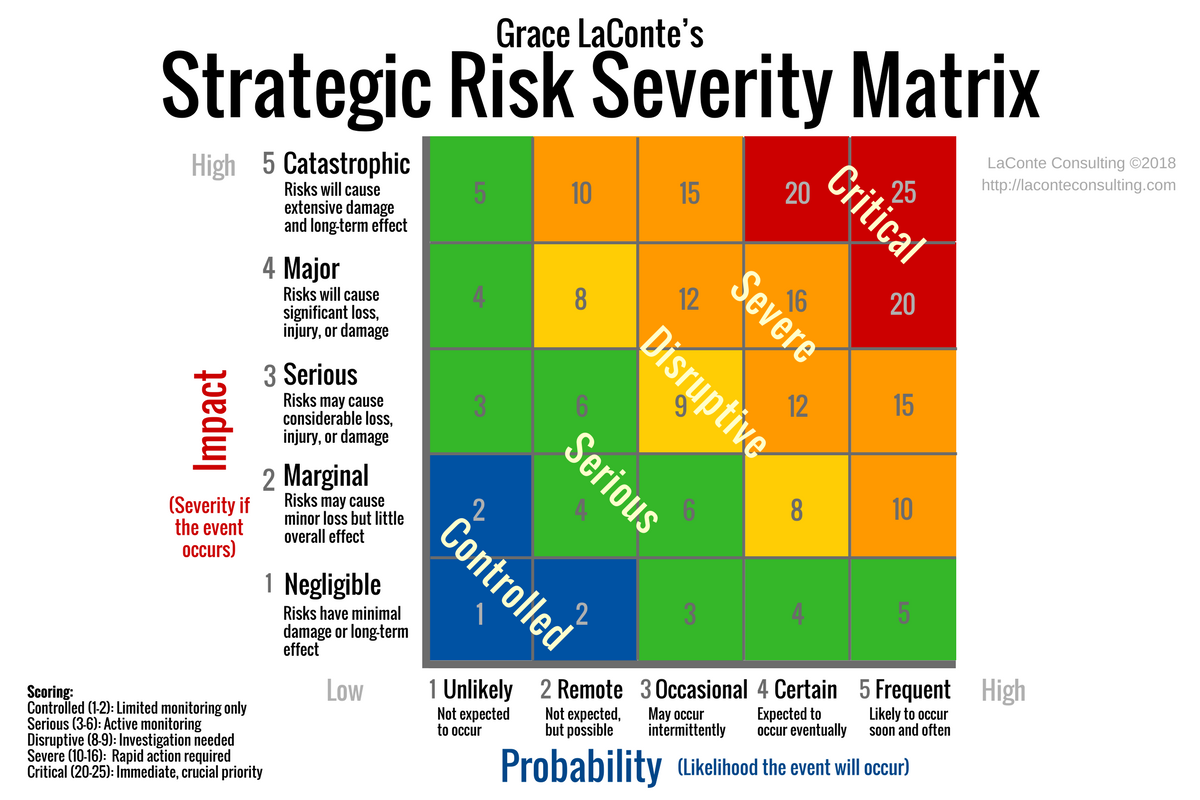
\includegraphics[height=.7\textheight]{5/risk-severity-matrix}

\end{frame}

\begin{frame}
  \frametitle{Aanbevelingen}

  \begin{columns}
    \begin{column}{.5\textwidth}
      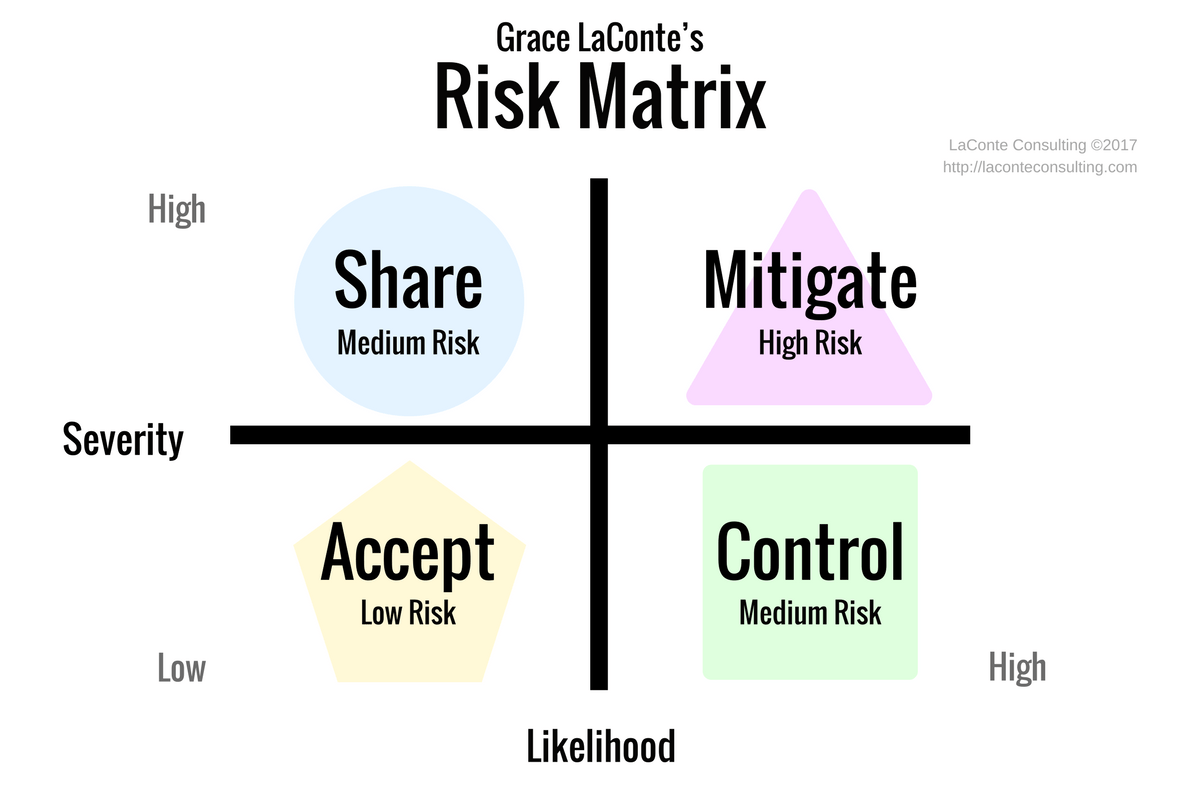
\includegraphics[width=\textwidth]{5/risk-matrix-severity-and-likelihood.png}
    \end{column}

    \begin{column}{.5\textwidth}
      \begin{itemize}
        \item \textbf{Mitigate:} Actie ondernemen, probleem oplossen
        \item \textbf{Control:} Transfereren naar andere entiteit (bv.\ uitbesteden naar IT service provider, securityspecialisten)
        \item \textbf{Share:} Verzekering nemen
        \item \textbf{Accept:} Niets doen
      \end{itemize}
    \end{column}
  \end{columns}

\end{frame}

\section{Proof of concept of testopstelling}

\begin{frame}
  \frametitle{Proof of concept/testopstelling}

  \begin{itemize}
    \item Doel:
          \begin{itemize}
            \item Aantonen dat voorgestelde oplossing realiseerbaar is
            \item Opstelling voor uitvoeren experimenten
          \end{itemize}
    \item Belangrijke eigenschappen:
          \begin{itemize}
            \item Reproduceerbaarheid
            \item Repliceerbaarheid
            \item Herbruikbaarheid
          \end{itemize}
  \end{itemize}

\end{frame}

\begin{frame}
  \frametitle{Reproduceerbaarheid}

  \alertbox{Geef de lezer voldoende info om jouw testopstelling te reproduceren}

  \bigskip

  \begin{itemize}
    \item Welke hardware? Specs?
          \begin{itemize}
            \item Computers, netwerkapparatuur, \ldots
          \end{itemize}
    \item Welke software?
    \item Installatie- en configuratie?
    \item Voeg afbeelding toe met schema testopstelling!
  \end{itemize}

\end{frame}

\begin{frame}
  \frametitle{Repliceerbaarheid}

  \alertbox{De lezer moet jouw opstelling snel opnieuw kunnen opzetten}

  \bigskip

  \begin{itemize}
    \item Gedetailleerde procedurehandleiding
    \item Automatiseren! Bv.\ Vagrant, Docker\ldots
    \item Installatiescript, configbestanden, docs\ldots\ in GitHub-repo!
  \end{itemize}

\end{frame}

\begin{frame}
  \frametitle{Herbruikbaarheid}

  \alertbox{Je kan gelijkaardige varianten van een testopstelling creëren}

  \bigskip

  \begin{itemize}
    \item Vergelijken alternatieven
    \item Vergelijken verschillen in configuratie
  \end{itemize}

\end{frame}

\section{Kwantitatieve data}

\begin{frame}
  \frametitle{Kwantitatieve data verzamelen}

  Bv.\ performatiemetingen

  \begin{itemize}
    \item Reproduceerbaar, repliceerbaar, herbruikbaar
    \item Automatiseer experimenten (bv.\ shellscript)
    \item Sla resultaten op in bruikbaar formaat
          \begin{itemize}
            \item Tekstgebaseerd
            \item Computer readable
            \item bv.\ CSV, JSON, YAML
          \end{itemize}
  \end{itemize}

\end{frame}

\begin{frame}
  \frametitle{Kwantitatieve data verwerken}

  \begin{itemize}
    \item Gebruik statistische software (Python, R)
    \item Geschikte visualisatie- en analysetechnieken
          \begin{itemize}
            \item Zie Data Science \& AI!
            \item Toon spreiding in de data
            \item Pas statistische toetsen toe
          \end{itemize}
  \end{itemize}

\end{frame}

\begin{frame}
  \frametitle{Bivariate analysis: overview}
  \centering
  \begin{tabular}{lll}
    \toprule
    \textbf{Independent} & \textbf{Dependent} & \textbf{Test/Metric}    \\
    \midrule
    Qualitative          & Qualitative        & $\chi^2$-test           \\
                         &                    & Cramér's $V$            \\
    Qualitative          & Quantitative       & two-sample $t$-test     \\
                         &                    & Cohen's $d$             \\
    Quantitative         & Quantitative       & Regression, correlation \\
    \bottomrule
  \end{tabular}

  \bigskip

  \alertbox{Er zijn nog meer statistische technieken dan we in DSAI gezien hebben!}
\end{frame}

\begin{frame}
  \frametitle{Kwantitatieve data verwerken}

  Stel: onderzoeksvraag is `Welk DB-systeem heeft de beste performantie: A of B?'

  \begin{itemize}
    \item<+-> Welk experiment ga je opzetten?
      % Testopstelling met DB A en B
      % Herhaald queries uitvoeren op A en B, tijd meten
    \item<+-> Wat zijn de onafhankelijke en afhankelijke variabele?
      % Onafh: DB-systeem (A of B)
      % Afh: responstijd
    \item<+-> Met welk soort grafiek zou je dit visualiseren?
      % Boxplot, dichtheidsdiagram (kdeplot)
      % Staafdiagram van gemiddelden? ENKEL ALS JE OOK SPREIDING TOONT ahv error bars, maar dit is enkel zinvol als data duidelijk normaal verdeeld is
    \item<+-> Met welke techniek kan je de onderzoeksvraag beantwoorden?
      % t-toets voor 2 onafhankelijke steekproeven
  \end{itemize}

\end{frame}

\begin{frame}
  \frametitle{Tips bij verwerken data}

  \begin{itemize}
    \item Ruwe data (CSV) NOOIT wijzigen
    \item Automatiseer zoveel mogelijk de workflow
          \begin{itemize}
            \item Python script of Jupyter Notebook
            \item Import CSV
            \item Data cleaning
            \item Visualisatie
            \item Analyse
          \end{itemize}
    \item Hou je code bij in Git!
  \end{itemize}

  \alertbox{Denk aan reproduceerbaarheid en repliceerbaarheid!}

\end{frame}

\section{Valkuil: de enquête}

\begin{frame}
  \frametitle{De enquête}

  \alertbox{Voor een BP Toegepaste Informatica is een enquête meestal af te raden!}

  \bigskip

  \begin{itemize}
    \item Vaak ongeschikt voor beantwoorden onderzoeksvraag
    \item Vaak te weinig respondenten
    \item Vaak onbruikbare resultaten
  \end{itemize}

\end{frame}

\begin{frame}
  \frametitle{Een goede steekproef}

  Zie ook Data Science \& AI

  \begin{itemize}
    \item Goed gedefinieerde populatie (steekproefkader!)
    \item Aselect
    \item Voldoende groot
    \item Representatief (gestratificeerd)
  \end{itemize}

\end{frame}

\begin{frame}
  \frametitle{Vaak voorkomende problemen}

  \begin{itemize}
    \item Populatie is niet/slecht gedefinieerd
    \item Steekproef is niet aselect
          \begin{itemize}
            \item online enquête
            \item convenience sampling
          \end{itemize}
    \item Zeer laag responspercentage
    \item Ondoordachte vragen $\Rightarrow$ onbruikbare antwoorden
          \begin{itemize}
            \item Open vragen
            \item Peilen naar opinie, geen feiten
          \end{itemize}
    \item Geen controle op representativiteit
  \end{itemize}

\end{frame}

\section{Vervolg opdracht}

\begin{frame}
  \frametitle{Uitschrijven methodologie}

  \begin{itemize}
    \item Schrijf plan van aanpak uit (= methodologie)
    \item Verdeel onderzoek in verschillende fasen
          \begin{itemize}
            \item Wat ga je concreet doen?
            \item Waarom? Wat is de doelstelling?
            \item Wat is het concrete resultaat?
            \item Hoe ga je het aanpakken (onderzoeksmethode)?
          \end{itemize}
    \item Schatting tijdverloop (normale BP):
          \begin{itemize}
            \item Begin: start semester 2
            \item Per week 4d stage, 1d BP (géén paasvakantie!)
            \item Deadline: vrijdag eerste examenweek
          \end{itemize}
  \end{itemize}

\end{frame}

\end{document}
